%% ============================================================================
%% Guia Técnico: Evolução Autônoma do Ecossistema OpenCode
%% Formato ABNT NBR 6022:2018 — Artigo Científico
%% Compilação: pdflatex → bibtex → pdflatex → pdflatex
%% ============================================================================

\documentclass[
  article,
  12pt,
  oneside,
  a4paper,
  brazil,
  sumario=tradicional
]{abntex2}

% --- Pacotes Fundamentais ---
\usepackage[utf8]{inputenc}
\usepackage[T1]{fontenc}
\usepackage{lmodern}
\usepackage{indentfirst}
\usepackage{graphicx}
\usepackage{xcolor}
\usepackage{microtype}
\usepackage{amsmath}
\usepackage{amssymb}
\usepackage{float}
\usepackage{placeins}
\usepackage{tcolorbox}
\usepackage{xurl}
\tcbuselibrary{breakable}

% --- Controle de hifenização e margens ---
\emergencystretch=1.5em
\tolerance=500
\pretolerance=200
\hyphenation{eco-ssis-te-ma Open-Code Ma-nus E-vol-ve Au-to-E-vol-ve me-to-do-lo-gi-a o-pe-ra-cio-nal ve-ri-fi-ca-do-res or-ques-tra-dor sin-cro-ni-za-ção va-li-da-ção trans-for-ma-ções com-po-nen-tes es-pe-ci-a-li-za-dos au-to-ma-ti-ca-men-te do-cu-men-ta-dos con-fi-a-bi-li-da-de a-gen-te}

% --- Caixas didáticas "Para Entender Melhor" ---
\definecolor{leigosbg}{RGB}{255,252,240}
\definecolor{leigosframe}{RGB}{180,140,40}
\newtcolorbox{leigosbox}[1][]{
  colback=leigosbg,
  colframe=leigosframe,
  fonttitle=\bfseries\small,
  before upper={\raggedright\footnotesize},
  title={\Large\color{leigosframe}?}\; \textbf{Para Entender Melhor},
  before skip=10pt,
  after skip=10pt,
  left=6pt,
  right=6pt,
  top=3pt,
  bottom=3pt,
  sharp corners,
  boxrule=0.6pt,
  breakable,
  #1
}

\definecolor{resumobg}{RGB}{245,248,255}
\definecolor{resumoframe}{RGB}{60,100,180}
\newtcolorbox{resumobox}{
  colback=resumobg,
  colframe=resumoframe,
  fonttitle=\bfseries\small,
  before upper={\raggedright\footnotesize},
  title={\Large\color{resumoframe}$\blacktriangleright$}\; \textbf{Em Resumo},
  before skip=10pt,
  after skip=10pt,
  left=6pt,
  right=6pt,
  top=3pt,
  bottom=3pt,
  sharp corners,
  boxrule=0.6pt,
  breakable
}

% --- Citações ABNT ---
\usepackage[brazilian,hyperpageref]{backref}
\usepackage[num,overcite]{abntex2cite}

\renewcommand{\backrefpagesname}{Citado na(s) página(s):~}
\renewcommand{\backref}{}
\renewcommand*{\backrefalt}[4]{%
  \ifcase #1 Nenhuma citação no texto.%
  \or Citado na página #2.%
  \else Citado #1 vezes nas páginas #2.%
  \fi}

% --- Configuração do PDF ---
\definecolor{blue}{RGB}{41,5,195}
\makeatletter
\hypersetup{
  pdftitle={Evolução Autônoma do Ecossistema OpenCode},
  pdfauthor={Marcelo Claro Laranjeira},
  pdfsubject={Engenharia de Software com Agentes Inteligentes},
  pdfcreator={LaTeX with abnTeX2},
  pdfkeywords={agentes inteligentes}{evolução autônoma}{orquestração}{multi-agente}{OpenCode},
  colorlinks=true,
  linkcolor=blue,
  citecolor=blue,
  filecolor=magenta,
  urlcolor=blue,
  bookmarksdepth=4
}
\makeatother

% --- Flowcharts: TikZ ---
\usepackage{tikz}
\usetikzlibrary{
  positioning,
  arrows.meta,
  shapes.geometric,
  shapes.multipart,
  backgrounds,
  fit,
  calc,
  matrix,
  chains
}

% --- Cores cyberpunk/esquemáticas ---
\definecolor{boxbg}{RGB}{240,245,255}
\definecolor{boxborder}{RGB}{41,98,255}
\definecolor{phasebg}{RGB}{255,248,240}
\definecolor{phaseborder}{RGB}{255,152,0}
\definecolor{skillbg}{RGB}{240,255,240}
\definecolor{skillborder}{RGB}{56,142,60}
\definecolor{agentbg}{RGB}{255,240,250}
\definecolor{agentborder}{RGB}{194,24,91}
\definecolor{reasonbg}{RGB}{250,245,255}
\definecolor{reasonborder}{RGB}{123,31,162}
\definecolor{arrowcolor}{RGB}{66,66,66}
\definecolor{stagebg}{RGB}{245,245,255}
\definecolor{stageborder}{RGB}{25,118,210}

% Estilos TikZ
\tikzset{
  procbox/.style={
    draw=boxborder, fill=boxbg, rounded corners=4pt,
    minimum width=5.8cm, minimum height=0.9cm,
    font=\footnotesize, align=center, text width=5.4cm
  },
  phasebox/.style={
    draw=phaseborder, fill=phasebg, rounded corners=4pt,
    minimum width=3.8cm, minimum height=0.8cm,
    font=\footnotesize\bfseries, align=center
  },
  skillnode/.style={
    draw=skillborder, fill=skillbg, rounded corners=3pt,
    minimum width=4.2cm, minimum height=0.7cm,
    font=\footnotesize, align=center, text width=3.8cm
  },
  agentnode/.style={
    draw=agentborder, fill=agentbg, rounded corners=3pt,
    minimum width=4.2cm, minimum height=0.7cm,
    font=\footnotesize, align=center, text width=3.8cm
  },
  reasonnode/.style={
    draw=reasonborder, fill=reasonbg, rounded corners=3pt,
    minimum width=4.2cm, minimum height=0.7cm,
    font=\footnotesize, align=center, text width=3.8cm
  },
  bigarrow/.style={
    ->, >=Stealth, line width=1.0pt, draw=arrowcolor
  },
  labelarrow/.style={
    ->, >=Stealth, line width=0.7pt, draw=arrowcolor, dashed
  },
  stagenode/.style={
    draw=stageborder, fill=stagebg, rounded corners=5pt,
    minimum width=2.6cm, minimum height=0.65cm,
    font=\footnotesize\bfseries, align=center
  },
  layernode/.style={
    draw=black!60, fill=black!3, rounded corners=6pt,
    minimum width=12cm,
    font=\footnotesize, align=center
  }
}

% Margens
\setlrmarginsandblock{2.5cm}{2.5cm}{*}
\setulmarginsandblock{2.5cm}{2.5cm}{*}
\checkandfixthelayout

\setlength{\parindent}{1.25cm}
\setlength{\parskip}{0.15cm}
\SingleSpacing

% --- Metadados ---
\titulo{Evolução Autônoma de Ecossistemas de Agentes Inteligentes:\\
Metodologia Técnica de Geração Automática de \emph{Skills}, Agentes e Raciocínios Orquestrados no Framework OpenCode}
\tituloestrangeiro{Autonomous Evolution of Intelligent Agent Ecosystems: Technical Methodology for Automatic Generation of Skills, Agents, and Orchestrated Reasoning in the OpenCode Framework}

\autor{Marcelo Claro Laranjeira\thanks{Pesquisador independente. Ecossistema OpenCode v5.0. E-mail: \texttt{marcelo@opencode.ai}}}

\local{Fortaleza, Ceará}
\data{Junho de 2026}

\makeindex

\begin{document}

\selectlanguage{brazil}
\frenchspacing
\maketitle

% =============================================================================
% RESUMO
% =============================================================================
\begin{resumoumacoluna}
Este artigo apresenta a metodologia técnica completa para evolução autônoma do ecossistema OpenCode --- um framework de inteligência artificial baseado em agentes múltiplos que implementa geração automática de \emph{skills}, agentes especializados e raciocínios orquestrados. A arquitetura opera em seis camadas interdependentes: (1) plugin \emph{Manus Evolve} em TypeScript que captura padrões de uso via hooks de ciclo de vida com pipeline PLAN--ACT--CORRECT--REFLECT--EXTRACT--EVOLVE; (2) agente \emph{AutoEvolve} que descobre e instala componentes externos via SENSE--DISCOVER--INSTALL--VERIFY--EVOLVE--LEARN; (3) \emph{Evolution Loop} em Python com ciclo fechado DETECT--DIAGNOSE--HEAL--LEARN--EVOLVE--INTEGRATE e agentes de diagnóstico multi-perspectiva; (4) \emph{Sync Orchestrator} que mantém matriz de validação cruzada com mais de 200 afinidades e \emph{health scoring} dinâmico; (5) \emph{Evolution Optimizer} com \emph{fitness scoring} multi-critério e mutação adaptativa; e (6) \emph{MiroFish Sync} que monitora repositórios \emph{upstream} para extrair novos padrões. O sistema acumulou 14 ciclos documentados de evolução com pontuações de 85 a 98/100. A fundamentação teórica apoia-se em arquiteturas multiagente \cite{wu2023autogen}, agentes generativos com memória e reflexão \cite{park2023generative,shinn2023reflexion}, \emph{chain-of-thought prompting} \cite{wei2022chainofthought}, projeto automatizado de sistemas agentivos \cite{hu2024adas}, e verificação formal via \emph{SMT solving} \cite{demoura2008z3}.

\vspace{\onelineskip}
\noindent\textbf{Palavras-chave}: Agentes inteligentes. Evolução autônoma. Orquestração multiagente. Geração automática de habilidades. Verificação formal. Ecossistema de software. OpenCode.
\end{resumoumacoluna}

\begin{resumoumacoluna}
\begin{otherlanguage*}{english}
This paper presents the complete technical methodology for autonomous evolution of the OpenCode ecosystem --- a multi-agent artificial intelligence framework implementing automatic generation of skills, specialized agents, and orchestrated reasoning. The architecture operates on six interdependent layers: (1) Manus Evolve TypeScript plugin capturing usage patterns via lifecycle hooks with a PLAN--ACT--CORRECT--REFLECT--EXTRACT--EVOLVE pipeline; (2) AutoEvolve agent discovering and installing external components via SENSE--DISCOVER--INSTALL--VERIFY--EVOLVE--LEARN; (3) Python Evolution Loop with closed-cycle DETECT--DIAGNOSE--HEAL--LEARN--EVOLVE--INTEGRATE and multi-perspective diagnostic agents; (4) Sync Orchestrator maintaining a cross-validation matrix with 200+ affinities and dynamic health scoring; (5) Evolution Optimizer with multi-criteria fitness scoring and adaptive mutation; and (6) MiroFish Sync monitoring upstream repositories to extract new patterns. The system accumulated 14 documented evolution cycles with scores from 85 to 98/100. Theoretical foundations rest on multi-agent architectures, generative agents with memory and reflection, chain-of-thought prompting, automated design of agentic systems, and formal verification via SMT solving.

\vspace{\onelineskip}
\noindent\textbf{Keywords}: Intelligent agents. Autonomous evolution. Multi-agent orchestration. Automatic skill generation. Formal verification. Software ecosystem. OpenCode.
\end{otherlanguage*}
\end{resumoumacoluna}

% =============================================================================
% TEXTO
% =============================================================================
\textual

% =============================================================================
% 1. INTRODUÇÃO
% =============================================================================
\section{Introdução}

Ecossistemas de software baseados em inteligência artificial enfrentam um desafio estrutural: como evoluir autonomamente sem intervenção humana constante, gerando novos componentes (\emph{skills}), novos atores (agentes) e novas capacidades de raciocínio de forma coordenada e verificável. O framework OpenCode aborda esse problema com uma arquitetura de evolução autônoma em seis camadas, que opera sobre um ecossistema de mais de 600 componentes integrados --- incluindo 46 MCPs \emph{(Model Context Protocol)}, 150 \emph{skills}, 125 agentes e 212 tipos de raciocínio catalogados em 27 categorias.

A arquitetura fundamenta-se em três pilares teóricos: (i) sistemas multiagente com orquestração autônoma, conforme demonstrado por \citeonline{wu2023autogen} no framework AutoGen e por \citeonline{park2023generative} em agentes generativos com arquitetura de memória-reflexão-planejamento; (ii) ciclos de auto-aperfeiçoamento iterativo, inspirados no mecanismo de \emph{verbal reinforcement learning} do Reflexion \cite{shinn2023reflexion} e no auto-refinamento com \emph{self-feedback} de \citeonline{madaan2023selfrefine}; e (iii) verificação formal de correção, apoiada em \emph{SMT solving} via Z3 \cite{demoura2008z3} e computação simbólica via SymPy \cite{meurer2017sympy}.

Este guia apresenta a metodologia técnica completa --- passo a passo --- para operar o pipeline de evolução do ecossistema OpenCode, com ênfase na geração automática de \emph{skills} reutilizáveis, na criação de novos agentes especializados e na orquestração de raciocínios verificáveis.

\begin{leigosbox}
\textbf{O problema em linguagem simples.} Imagine uma grande empresa com 600 funcionários, cada um com uma especialidade diferente. Todo dia, novos problemas surgem e a empresa precisa: (a) treinar novos funcionários (agentes) para resolver esses problemas; (b) criar manuais de procedimento (skills) para que o conhecimento não se perca; e (c) melhorar a forma de pensar sobre os problemas (raciocínios). Fazer tudo isso \textbf{manualmente} demandaria um exército de gerentes. O OpenCode resolve esse problema com \textbf{6 robôs-gerentes} que trabalham juntos --- cada um responsável por uma etapa do processo --- para que o ecossistema \textbf{evolua sozinho}, aprendendo com seus próprios erros e acertos, como um organismo vivo.
\end{leigosbox}

% =============================================================================
% 2. ARQUITETURA DO ECOSSISTEMA
% =============================================================================
\section{Arquitetura do Ecossistema OpenCode}

O ecossistema OpenCode opera em uma arquitetura de três camadas (MCP $\rightarrow$ Skill $\rightarrow$ Agente), sobre a qual se sobrepõem seis motores de evolução autônoma. A Figura~\ref{fig:arquitetura} apresenta o diagrama arquitetural completo.

\begin{figure}[H]
  \centering
  \begin{tikzpicture}[
    node distance=0.4cm and 0.5cm,
    every node/.style={align=center}
  ]

    % EXTERNAL SOURCES (top)
    \node[layernode, fill=black!2, minimum height=1.0cm, minimum width=11cm] (externals) {
      \textbf{Fontes Externas}\\[1pt]
      \fontsize{5}{6}\selectfont\texttt{github.com/666ghj/MiroFish $\cdot$ github.com/666ghj/BettaFish}\\[0pt]
      \fontsize{5}{6}\selectfont\texttt{github.com/bytedance/deer-flow}
    };

    % 6 EVOLUTION ENGINES
    \node[layernode, below=0.3cm of externals, fill=phasebg!30, draw=phaseborder, minimum height=1.3cm, minimum width=11cm] (engines) {
      \textbf{6 Motores de Evolução Autônoma} \\[2pt]
      \begin{tikzpicture}[node distance=0.15cm and 0.2cm]
        \node[stagenode, minimum width=1.7cm, font=\fontsize{5}{6}\selectfont\bfseries] (e1) {Manus Evolve};
        \node[stagenode, minimum width=1.7cm, font=\fontsize{5}{6}\selectfont\bfseries, right=of e1] (e2) {AutoEvolve};
        \node[stagenode, minimum width=1.7cm, font=\fontsize{5}{6}\selectfont\bfseries, right=of e2] (e3) {Evolution Loop};
        \node[stagenode, minimum width=1.7cm, font=\fontsize{5}{6}\selectfont\bfseries, below=of e1] (e4) {Sync Orch.};
        \node[stagenode, minimum width=1.7cm, font=\fontsize{5}{6}\selectfont\bfseries, right=of e4] (e5) {Evo Optimizer};
        \node[stagenode, minimum width=1.7cm, font=\fontsize{5}{6}\selectfont\bfseries, right=of e5] (e6) {MiroFish Sync};
      \end{tikzpicture}
    };

    % MAIN ARCHITECTURE
    \node[layernode, below=0.3cm of engines, fill=boxbg!40, draw=boxborder, minimum height=3.5cm, minimum width=11cm] (core) {
      \textbf{Arquitetura Core: 3 Camadas} \\[3pt]
      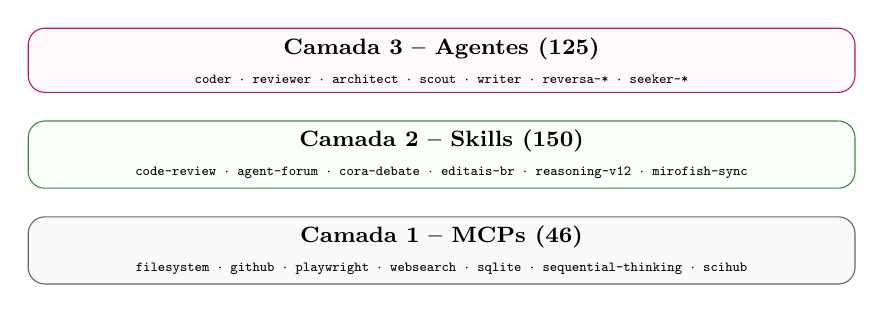
\begin{tikzpicture}[node distance=0.35cm]
        \node[layernode, fill=agentbg!30, draw=agentborder, minimum width=10.5cm, minimum height=0.8cm] (agents) {
          \textbf{Camada 3 -- Agentes (125)}\\[1pt]
          \fontsize{5}{6}\selectfont\texttt{coder $\cdot$ reviewer $\cdot$ architect $\cdot$ scout $\cdot$ writer $\cdot$ reversa-* $\cdot$ seeker-*}
        };
        \node[layernode, fill=skillbg!30, draw=skillborder, minimum width=10.5cm, minimum height=0.8cm, below=of agents] (skills) {
          \textbf{Camada 2 -- Skills (150)}\\[1pt]
          \fontsize{5}{6}\selectfont\texttt{code-review $\cdot$ agent-forum $\cdot$ cora-debate $\cdot$ editais-br $\cdot$ reasoning-v12 $\cdot$ mirofish-sync}
        };
        \node[layernode, fill=black!2, minimum width=10.5cm, minimum height=0.8cm, below=of skills] (mcps) {
          \textbf{Camada 1 -- MCPs (46)}\\[1pt]
          \fontsize{5}{6}\selectfont\texttt{filesystem $\cdot$ github $\cdot$ playwright $\cdot$ websearch $\cdot$ sqlite $\cdot$ sequential-thinking $\cdot$ scihub}
        };
      \end{tikzpicture}
    };

    % OUTPUTS
    \node[layernode, below=0.3cm of core, fill=reasonbg!30, draw=reasonborder, minimum height=1.3cm, minimum width=11cm] (outputs) {
      \textbf{Saídas Evolutivas} \\[2pt]
      
\begin{tikzpicture}[node distance=0.2cm and 0.6cm]
        \node[skillnode, minimum width=3.2cm, font=\fontsize{5}{6}\selectfont] (s1) {\textbf{Skills}\\\texttt{evolution/evo-*.md}};
        \node[agentnode, minimum width=3.2cm, font=\fontsize{5}{6}\selectfont, right=of s1] (s2) {\textbf{Agentes}\\\texttt{agents/*.md}};
        \node[reasonnode, minimum width=3.2cm, font=\fontsize{5}{6}\selectfont, right=of s2] (s3) {\textbf{Raciocínios}\\\texttt{212 tipos / 27 cat.}};
      \end{tikzpicture}
    };

    \draw[bigarrow] (externals.south) -- (engines.north);
    \draw[bigarrow] (engines.south) -- (core.north);
    \draw[bigarrow] (core.south) -- (outputs.north);

  \end{tikzpicture}
  \caption{Arquitetura do ecossistema OpenCode: 6 motores de evolução autônoma atuando sobre 3 camadas core, com fontes externas de padrões e saídas evolutivas.}
  \label{fig:arquitetura}
  \legend{Fonte: Elaboração própria baseada na documentação do ecossistema OpenCode v5.0.}
\end{figure}

A arquitetura segue o princípio de separação de responsabilidades em camadas, conforme os padrões de projeto para sistemas de software \cite{gamma1994design}. Cada camada comunica-se exclusivamente com suas adjacentes, e os motores de evolução atuam transversalmente como \emph{aspectos} que interceptam o fluxo normal de operação --- análogo ao conceito de \emph{pipeline} de CI/CD contínuo \cite{bass2021devops}.

\begin{leigosbox}
\textbf{A anatomia do ecossistema --- a casa de três andares.} Pense no OpenCode como uma casa com três andares e seis sistemas inteligentes que a mantêm funcionando:

\vspace{2pt}
\noindent\textbf{Térreo -- Ferramentas (46 MCPs).} São os \emph{equipamentos} da casa: sistema elétrico, encanamento, acesso à internet. Sem eles, nada funciona. Exemplos: acesso a arquivos, busca na web, bancos de dados, navegador.

\vspace{2pt}
\noindent\textbf{1.\textsuperscript{o} Andar -- Manuais (150 Skills).} São os \emph{procedimentos operacionais}: ``como revisar código'', ``como buscar editais'', ``como verificar fatos''. Cada skill é um conhecimento encapsulado e reutilizável.

\vspace{2pt}
\noindent\textbf{2.\textsuperscript{o} Andar -- Funcionários (125 Agentes).} São os \emph{executores} que usam as ferramentas do térreo seguindo os manuais do 1.\textsuperscript{o} andar para realizar tarefas complexas.

\vspace{4pt}
\noindent Os \textbf{6 motores de evolução} são como uma \emph{equipe de facilities} 24h: um vigia novos manuais na internet, outro conserta falhas, outro aprende com erros, outro conecta tudo. O resultado: a casa \textbf{se constrói e se reforma sozinha}.
\end{leigosbox}

% =============================================================================
% 3. FUNDAMENTAÇÃO TEÓRICA
% =============================================================================
\section{Fundamentação Teórica}

\subsection{Sistemas Multiagente com Orquestração Autônoma}

O paradigma multiagente aplicado a \emph{Large Language Models} (LLMs) -- cuja arquitetura \emph{Transformer} foi estabelecida por \citeonline{vaswani2017attention} --- evoluiu rapidamente desde 2023. O framework AutoGen \cite{wu2023autogen} demonstrou que agentes LLM podem coordenar-se autonomamente em conversações multi-turno, com papéis especializados e troca de artefatos. Os agentes generativos de \citeonline{park2023generative} estabeleceram a arquitetura de memória-reflexão-planejamento que inspira o ciclo PLAN--ACT--REFLECT do Manus Evolve. O CAMEL \cite{li2023camel} introduziu o conceito de \emph{role-playing} autônomo entre agentes para exploração colaborativa de problemas.

\subsection{Ciclos de Auto-Aperfeiçoamento Iterativo}

O mecanismo de \emph{Reflexion} \cite{shinn2023reflexion} demonstrou que agentes podem aprender com \emph{feedback} verbal em loop, melhorando seu desempenho sem atualização de pesos. O \emph{Self-Refine} \cite{madaan2023selfrefine} estendeu esse conceito para auto-refinamento iterativo via \emph{feedback} do próprio LLM. O Voyager \cite{wang2023voyager} mostrou que agentes podem gerar e aperfeiçoar autonomamente currículos de habilidades (\emph{skill libraries}), princípio que fundamenta a geração de \emph{skills} no diretório \texttt{evolution/}.

O \emph{Automated Design of Agentic Systems} (ADAS) \cite{hu2024adas} constitui o fundamento mais direto: um meta-agente que projeta automaticamente novos sistemas agentivos via busca em espaço de código, com \emph{fitness scoring} multi-critério --- mesma abordagem do \emph{Evolution Optimizer} do OpenCode.

\subsection{Verificação Formal e Raciocínio Orquestrado}

O \emph{Chain-of-Thought} \cite{wei2022chainofthought} demonstrou que LLMs podem decompor raciocínio complexo em etapas encadeadas. O \emph{Tree of Thoughts} \cite{yao2023treeofthoughts} expandiu para exploração de múltiplos caminhos com poda. O debate multiagente como mecanismo de verificação foi validado por \citeonline{du2023improving}.

Para verificação formal de correção, o Z3 \cite{demoura2008z3} fornece \emph{Satisfiability Modulo Theories} (SMT) \emph{solving} para validação de pré/pós-condições nos \emph{barriers} de sincronização. O SymPy \cite{meurer2017sympy} provê computação simbólica para validação de invariantes algébricos nos pipelines de raciocínio.

\begin{leigosbox}
\textbf{Os três pilares explicados com um exemplo cotidiano.} Suponha que você quer \textbf{cozinhar um jantar para 20 pessoas}. Como garantir que tudo dê certo?

\begin{enumerate}
\item[\textbf{Pilar 1}] \textbf{Múltiplos cozinheiros coordenados.} Em vez de um único chef sobrecarregado, você monta uma brigada: um no fogão, um nas saladas, um na sobremesa. Eles se comunicam entre si (``preciso do forno a 180\textdegree{} em 5 minutos''). É assim que o \textbf{AutoGen} e os \textbf{agentes generativos} funcionam --- cada agente cuida de uma parte e todos se coordenam.

\item[\textbf{Pilar 2}] \textbf{Aprender com os erros sem repetir receitas.} Se o bolo queimou da última vez, você ajusta o tempo do forno na próxima. Não precisa mudar o livro de receitas inteiro --- só aquele parâmetro. É o que fazem o \textbf{Reflexion} e o \textbf{Self-Refine}: melhoram continuamente sem ``resetar'' tudo.

\item[\textbf{Pilar 3}] \textbf{Um fiscal que confere cada etapa.} Antes de servir o prato, um provador oficial verifica: está cozido? Tempero certo? Textura correta? Se algo falhou, volta para a cozinha. O \textbf{Z3} e o \textbf{SymPy} fazem esse papel de ``provador oficial'' --- mas em vez de provar comida, eles \textbf{provam matematicamente} que cada etapa do raciocínio da IA está correta.
\end{enumerate}
\end{leigosbox}

% =============================================================================
% 4. O PIPELINE DE EVOLUÇÃO — PASSO A PASSO
% =============================================================================
\section{O Pipeline de Evolução Autônoma: Procedimento Técnico}

O procedimento de evolução do ecossistema OpenCode compreende 8 (oito) passos sequenciais. A Figura~\ref{fig:pipeline} apresenta o fluxograma completo.

\begin{leigosbox}
\textbf{A rotina diária de um ecossistema que se auto-gerencia.} Imagine que você tem uma \textbf{fazenda inteligente} que se administra sozinha. Todo dia, ao amanhecer, ela executa uma rotina de 8 tarefas:

\begin{enumerate}
\item[\textbf{6h}] \textbf{Explorar} --- sai para ver se há novas sementes, ferramentas ou técnicas agrícolas disponíveis no mercado (Passo 1: \texttt{/evolve}).
\item[\textbf{7h}] \textbf{Vistoriar} --- percorre cada canteiro, cada galpão, cada cerca. Anota tudo que está quebrado ou fora do lugar (Passo 2: Scanner + Healer).
\item[\textbf{8h}] \textbf{Diagnosticar + Consertar} --- aciona a equipe de manutenção para corrigir os problemas encontrados. Se algo não tem solução automática, emite um alerta (Passo 3: Evolution Loop).
\item[\textbf{9h}] \textbf{Aprender} --- compara o estado de hoje com o de ontem, da semana passada, do mês passado. Identifica tendências: ``a cerca leste está enferrujando mais rápido que a oeste'' (Passo 4: Learn).
\item[\textbf{10h}] \textbf{Sincronizar} --- conecta os aprendizados da casa (TypeScript) com os do campo (Python) para que todos falem a mesma língua (Passo 5: Bridge).
\item[\textbf{11h}] \textbf{Check-up geral} --- mede a saúde de cada setor com uma nota de 0 a 100. Se algo estiver abaixo de 70, aciona reforço (Passo 6: Health Check).
\item[\textbf{12h}] \textbf{Relatório + Otimização} --- gera um boletim com tudo que foi feito e ajusta os pesos da avaliação para o dia seguinte (Passo 7: Report + Optimizer).
\item[\textbf{Semanal}] \textbf{Visita às fazendas vizinhas} --- vai até os repositórios MiroFish, BettaFish e DeerFlow para ver o que eles inventaram de novo e trazer para casa (Passo 8: MiroFish Sync).
\end{enumerate}

\noindent Tudo isso acontece \textbf{sem um gerente humano} dar cada ordem. A fazenda aprendeu a se gerenciar --- é assim que o OpenCode opera.
\end{leigosbox}

\begin{figure}[H]
  \centering
  \small
  \begin{tikzpicture}[
    node distance=0.35cm and 0.6cm,
    every node/.style={align=center}
  ]

    % Column 1: P1 + P5
    \node[phasebox, minimum width=3.2cm, font=\fontsize{7}{8}\selectfont\bfseries] (p1) {\texttt{/evolve}};
    \node[procbox, minimum height=1.1cm, minimum width=3.2cm, below=0.25cm of p1, font=\fontsize{6}{7}\selectfont, text width=3.0cm] (d1) {
      \textbf{Passo 1}\\[1pt]
      SENSE→DISCOVER\\
      INSTALL→VERIFY\\
      EVOLVE→LEARN
    };
    \node[phasebox, minimum width=3.2cm, font=\fontsize{7}{8}\selectfont\bfseries, below=0.5cm of d1] (p5) {Bridge TS\,$\leftrightarrow$\,PY};
    \node[procbox, minimum height=0.9cm, minimum width=3.2cm, below=0.25cm of p5, font=\fontsize{6}{7}\selectfont, text width=3.0cm] (d5) {
      \textbf{Passo 5}\\[1pt]
      bridge.py --sync --evolve
    };

    % Column 2: P2 + P6
    \node[phasebox, minimum width=3.2cm, font=\fontsize{7}{8}\selectfont\bfseries, right=of p1] (p2) {Scan + Heal};
    \node[procbox, minimum height=1.1cm, minimum width=3.2cm, below=0.25cm of p2, font=\fontsize{6}{7}\selectfont, text width=3.0cm] (d2) {
      \textbf{Passo 2}\\[1pt]
      scanner.py + healer.py\\
      --auto
    };
    \node[phasebox, minimum width=3.2cm, font=\fontsize{7}{8}\selectfont\bfseries, below=0.5cm of d2] (p6) {Health Check};
    \node[procbox, minimum height=0.9cm, minimum width=3.2cm, below=0.25cm of p6, font=\fontsize{6}{7}\selectfont, text width=3.0cm] (d6) {
      \textbf{Passo 6}\\[1pt]
      bridge.py health + orch.
    };

    % Column 3: P3 + P7
    \node[phasebox, minimum width=3.2cm, font=\fontsize{7}{8}\selectfont\bfseries, right=of p2] (p3) {Evo Loop};
    \node[procbox, minimum height=1.1cm, minimum width=3.2cm, below=0.25cm of p3, font=\fontsize{6}{7}\selectfont, text width=3.0cm] (d3) {
      \textbf{Passo 3}\\[1pt]
      DETECT→DIAGNOSE\\
      HEAL→LEARN\\
      EVOLVE→INTEGRATE
    };
    \node[phasebox, minimum width=3.2cm, font=\fontsize{7}{8}\selectfont\bfseries, below=0.5cm of d3] (p7) {Relatório};
    \node[procbox, minimum height=0.9cm, minimum width=3.2cm, below=0.25cm of p7, font=\fontsize{6}{7}\selectfont, text width=3.0cm] (d7) {
      \textbf{Passo 7}\\[1pt]
      --report + optim.py
    };

    % Column 4: P4 + P8
    \node[phasebox, minimum width=3.2cm, font=\fontsize{7}{8}\selectfont\bfseries, right=of p3] (p4) {Learn};
    \node[procbox, minimum height=1.1cm, minimum width=3.2cm, below=0.25cm of p4, font=\fontsize{6}{7}\selectfont, text width=3.0cm] (d4) {
      \textbf{Passo 4}\\[1pt]
      --learn + --suggest
    };
    \node[phasebox, minimum width=3.2cm, font=\fontsize{7}{8}\selectfont\bfseries, below=0.5cm of d4] (p8) {MiroFish Sync};
    \node[procbox, minimum height=0.9cm, minimum width=3.2cm, below=0.25cm of p8, font=\fontsize{6}{7}\selectfont, text width=3.0cm] (d8) {
      \textbf{Passo 8 (semanal)}\\[1pt]
      MONITOR→DIFF\\
      EXTRACT→INTEGRATE
    };

    % Arrows row 1: P1→P2→P3→P4
    \draw[bigarrow] (p1.east) -- (p2.west);
    \draw[bigarrow] (p2.east) -- (p3.west);
    \draw[bigarrow] (p3.east) -- (p4.west);

    % Arrows row 2: P5→P6→P7→P8 (reverse order: P8←P7←P6←P5)
    \draw[bigarrow] (p8.east) -- (p7.west);
    \draw[bigarrow] (p7.east) -- (p6.west);
    \draw[bigarrow] (p6.east) -- (p5.west);

    % Arrows: top→detail
    \draw[bigarrow] (p1.south) -- (d1.north);
    \draw[bigarrow] (p2.south) -- (d2.north);
    \draw[bigarrow] (p3.south) -- (d3.north);
    \draw[bigarrow] (p4.south) -- (d4.north);
    \draw[bigarrow] (p5.south) -- (d5.north);
    \draw[bigarrow] (p6.south) -- (d6.north);
    \draw[bigarrow] (p7.south) -- (d7.north);
    \draw[bigarrow] (p8.south) -- (d8.north);

  \end{tikzpicture}
  \caption{Fluxograma do pipeline de evolução autônoma em 8 passos, organizados em 4 colunas.}
  \label{fig:pipeline}
  \legend{Fonte: Elaboração própria baseada no ecossistema OpenCode v5.0.}
\end{figure}

\subsection{Passo 1: Ativação da Evolução Interativa (\texttt{/evolve})}

O comando \texttt{/evolve} aciona o agente \texttt{autoevolve.md}, que implementa o ciclo completo SENSE $\rightarrow$ DISCOVER $\rightarrow$ INSTALL $\rightarrow$ VERIFY $\rightarrow$ EVOLVE $\rightarrow$ LEARN:

\begin{alineas}
\item \textbf{SENSE}: auto-diagnóstico do ecossistema (lê \texttt{opencode.json}, \texttt{.evolve/\allowbreak memory.json}, lista \emph{skills}, \emph{plugins}, binários);
\item \textbf{DISCOVER}: busca em GitHub trending (\emph{topics/agent-skills}), marketplaces e atualizações pendentes (\texttt{npm outdated, pip list --outdated});
\item \textbf{INSTALL}: prioriza por \emph{stars}, compatibilidade e segurança; converte para OpenCode; registra em \texttt{installed.json};
\item \textbf{VERIFY}: valida \emph{frontmatter} YAML, conectividade MCP e binários;
\item \textbf{EVOLVE}: atualiza \emph{skills} com versão superior, remove componentes quebrados, consolida duplicatas;
\item \textbf{LEARN}: persiste métricas da sessão, atualiza \emph{ranking} de utilidade.
\end{alineas}

\subsection{Passo 2: Varredura e Auto-Cura (Scanner + Healer)}

O \emph{Ecosystem Scanner} (\texttt{ecosystem\_scanner.py}) varre todos os diretórios do ecossistema (\texttt{skills/}, \texttt{scripts/}, \texttt{plugins/}, \texttt{agents/}, \texttt{evals/}) e gera um manifesto JSON com anomalias detectadas. O \emph{Self Healer} (\texttt{self\_healer.py}) corrige automaticamente \emph{CJK leaks}, \emph{frontmatter} YAML ausente e erros de sintaxe em scripts Python.

\subsection{Passo 3: Ciclo de Evolução (Evolution Loop)}

O \emph{Evolution Loop} (\texttt{evolution\_loop.py}) executa o ciclo fechado de seis fases, documentado na Figura~\ref{fig:evoloop}.

\begin{figure}[H]
  \centering
  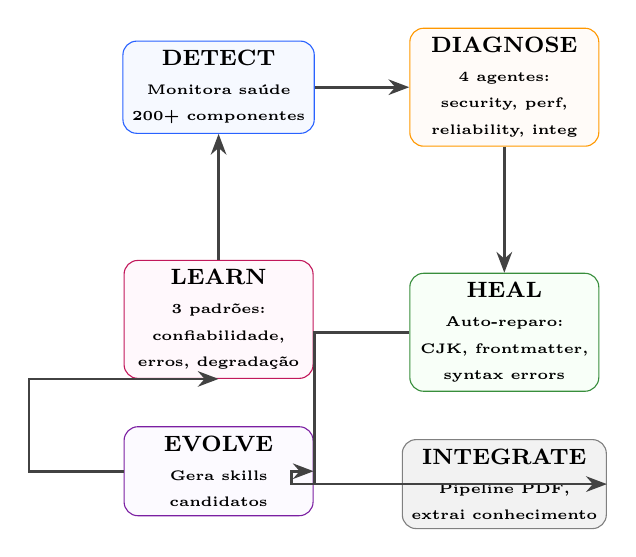
\begin{tikzpicture}[
    node distance=1.6cm and 1.2cm,
    every node/.style={align=center}
  ]
    % Central cycle - hexagon layout
    \node[stagenode, minimum width=2.4cm, fill=boxbg!60, draw=boxborder] (detect) {\textbf{DETECT}\\[1pt]\tiny Monitora saúde\\\tiny 200+ componentes};

    \node[stagenode, minimum width=2.4cm, fill=phasebg!50, draw=phaseborder, right=of detect] (diagnose) {\textbf{DIAGNOSE}\\[1pt]\tiny 4 agentes:\\\tiny security, perf,\\\tiny reliability, integ};

    \node[stagenode, minimum width=2.4cm, fill=skillbg!50, draw=skillborder, below=of diagnose] (heal) {\textbf{HEAL}\\[1pt]\tiny Auto-reparo:\\\tiny CJK, frontmatter,\\\tiny syntax errors};

    \node[stagenode, minimum width=2.4cm, fill=agentbg!50, draw=agentborder, below=of detect] (learn) {\textbf{LEARN}\\[1pt]\tiny 3 padrões:\\\tiny confiabilidade,\\\tiny erros, degradação};

    \node[stagenode, minimum width=2.4cm, fill=reasonbg!50, draw=reasonborder, below=0.6cm of learn] (evolve) {\textbf{EVOLVE}\\[1pt]\tiny Gera skills\\\tiny candidatos};

    \node[stagenode, minimum width=2.4cm, fill=black!5, draw=black!50, below=0.6cm of heal] (integrate) {\textbf{INTEGRATE}\\[1pt]\tiny Pipeline PDF,\\\tiny extrai conhecimento};

    % Arrow cycle
    \draw[bigarrow] (detect.east) -- (diagnose.west);
    \draw[bigarrow] (diagnose.south) -- (heal.north);
    \draw[bigarrow] (heal.west) -- ++(-1.2,0) |- (integrate.east);
    \draw[bigarrow] (integrate.west) -- ++(-1.4,0) |- (evolve.east);
    \draw[bigarrow] (evolve.west) -- ++(-1.2,0) |- (learn.south);
    \draw[bigarrow] (learn.north) -- (detect.south);

  \end{tikzpicture}
  \caption{Ciclo fechado do \emph{Evolution Loop}: DETECT $\rightarrow$ DIAGNOSE $\rightarrow$ HEAL $\rightarrow$ LEARN $\rightarrow$ EVOLVE $\rightarrow$ INTEGRATE.}
  \label{fig:evoloop}
  \legend{Fonte: Elaboração própria baseada em \texttt{evolution\_loop.py} (Nexus).}
\end{figure}

\subsection{Passo 4: Aprendizado Entre Ciclos}

O comando \texttt{evolution\_engine.py --learn} extrai padrões de melhoria e regressão entre \emph{snapshots} históricos armazenados em \texttt{cache/ecosystem\_history.json}, atualizando a base de conhecimento em \texttt{learnings.json} e \texttt{evolution\_knowledge.json}. O modo \texttt{--suggest} gera recomendações inteligentes classificadas por prioridade (alta, média, baixa).

\subsection{Passo 5: Ponte Manus Evolve (TypeScript) $\leftrightarrow$ Evolution Loop (Python)}

O script \texttt{manus\_evolve\_bridge.py} sincroniza os \emph{outcomes} registrados pelo plugin TypeScript (\texttt{.evolve/manus-state.json}) com o \texttt{FeedbackLoopEngine} Python. Cada \emph{round} do Manus é registrado como \texttt{LearningRecord} e o ciclo de evolução é disparado automaticamente.

\subsection{Passo 6: Health Check do Ecossistema}

O \texttt{ecosystem\_bridge.py health} monitora 8 componentes com pesos normalizados, verificando saúde de bancos de dados, \emph{embeddings}, agentes, scripts e integridade de diretórios. O \texttt{sync\_orchestrator.py} computa o \emph{health score} dinâmico e aciona auto-\emph{healing} quando necessário.

\subsection{Passo 7: Relatório e Otimização}

O \texttt{evolution\_engine.py --report} gera relatório Markdown de evolução. O \texttt{evolution\_optimizer.py} aplica \emph{fitness scoring} multi-critério com pesos: 30\% taxa de sucesso, 25\% velocidade, 20\% qualidade, 15\% eficiência de recursos e 10\% fator de inovação.

\subsection{Passo 8: Sincronização com Repositórios Externos (Semanal)}

O comando \texttt{/mirofish-sync} ativa o agente P19 que monitora três repositórios \emph{upstream} (MiroFish 61K $\star$, BettaFish 40.9K $\star$, DeerFlow) via GitHub API, extrai novos padrões via Reversa Scout e gera novas \emph{skills} P19+.

% =============================================================================
% 5. GERAÇÃO DE SKILLS
% =============================================================================
\section{Geração Automática de \emph{Skills}}

\emph{Skills} são o componente atômico de conhecimento no ecossistema OpenCode. Cada \emph{skill} é um arquivo Markdown com \emph{frontmatter} YAML contendo metadados de rastreabilidade. A Figura~\ref{fig:skillgen} ilustra as três vias de geração.

\begin{figure}[H]
  \centering
  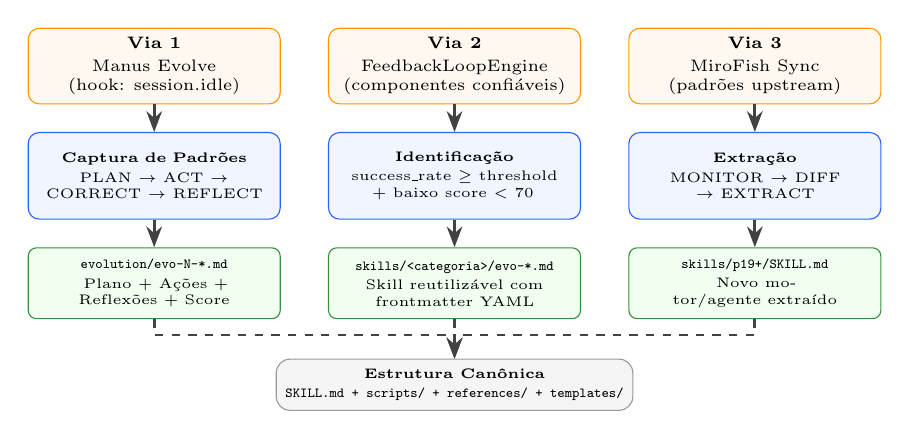
\begin{tikzpicture}[
    node distance=0.4cm and 0.6cm,
    every node/.style={align=center}
  ]

    \node[phasebox, minimum width=3.2cm, font=\fontsize{6}{7}\selectfont] (t1) {\textbf{Via 1}\\[1pt] Manus Evolve\\(hook: session.idle)};
    \node[phasebox, minimum width=3.2cm, font=\fontsize{6}{7}\selectfont, right=of t1] (t2) {\textbf{Via 2}\\[1pt] FeedbackLoopEngine\\(componentes confiáveis)};
    \node[phasebox, minimum width=3.2cm, font=\fontsize{6}{7}\selectfont, right=of t2] (t3) {\textbf{Via 3}\\[1pt] MiroFish Sync\\(padrões upstream)};

    \node[procbox, minimum height=1.1cm, minimum width=3.2cm, below=0.35cm of t1, font=\fontsize{5}{6}\selectfont, text width=2.8cm] (m1) {
      \textbf{Captura de Padrões}\\[1pt]
      PLAN $\rightarrow$ ACT $\rightarrow$\\
      CORRECT $\rightarrow$ REFLECT
    };
    \node[procbox, minimum height=1.1cm, minimum width=3.2cm, below=0.35cm of t2, font=\fontsize{5}{6}\selectfont, text width=2.8cm] (m2) {
      \textbf{Identificação}\\[1pt]
      success\_rate $\ge$ threshold\\
      + baixo score $<$ 70
    };
    \node[procbox, minimum height=1.1cm, minimum width=3.2cm, below=0.35cm of t3, font=\fontsize{5}{6}\selectfont, text width=2.8cm] (m3) {
      \textbf{Extração}\\[1pt]
      MONITOR $\rightarrow$ DIFF\\
      $\rightarrow$ EXTRACT
    };

    \draw[bigarrow] (t1) -- (m1);
    \draw[bigarrow] (t2) -- (m2);
    \draw[bigarrow] (t3) -- (m3);

    \node[skillnode, minimum height=0.9cm, minimum width=3.2cm, below=0.35cm of m1, font=\fontsize{5}{6}\selectfont, text width=2.8cm] (o1) {
      \textbf{\texttt{evolution/evo-N-*.md}}\\[1pt]
      Plano + Ações + Reflexões + Score
    };
    \node[skillnode, minimum height=0.9cm, minimum width=3.2cm, below=0.35cm of m2, font=\fontsize{5}{6}\selectfont, text width=2.8cm] (o2) {
      \textbf{\texttt{skills/<categoria>/evo-*.md}}\\[1pt]
      Skill reutilizável com frontmatter YAML
    };
    \node[skillnode, minimum height=0.9cm, minimum width=3.2cm, below=0.35cm of m3, font=\fontsize{5}{6}\selectfont, text width=2.8cm] (o3) {
      \textbf{\texttt{skills/p19+/SKILL.md}}\\[1pt]
      Novo motor/agente extraído
    };

    \draw[bigarrow] (m1) -- (o1);
    \draw[bigarrow] (m2) -- (o2);
    \draw[bigarrow] (m3) -- (o3);

    \node[stagenode, minimum width=4.5cm, fill=black!4, draw=black!40, below=0.5cm of o2, font=\fontsize{5}{6}\selectfont] (final) {\textbf{Estrutura Canônica}\\[1pt]\texttt{SKILL.md + scripts/ + references/ + templates/}};

    \draw[bigarrow, dashed] (o1.south) -- ++(0,-0.2) -| (final.north);
    \draw[bigarrow, dashed] (o2.south) -- (final.north);
    \draw[bigarrow, dashed] (o3.south) -- ++(0,-0.2) -| (final.north);

  \end{tikzpicture}
  \caption{Três vias de geração automática de \emph{skills} no ecossistema OpenCode, convergindo para a estrutura canônica padronizada.}
  \label{fig:skillgen}
  \legend{Fonte: Elaboração própria baseada em \texttt{manus-evolve.ts}, \texttt{evolution\_loop.py} e \texttt{mirofish-sync/SKILL.md}.}
\end{figure}

\subsection{Via 1: Manus Evolve (Plugin TypeScript)}

A cada evento \texttt{session.idle}, o plugin calcula um \emph{score} do \emph{round}:

\begin{equation}
S_{\text{round}} = \min(100,\ d \times 15 + k \times 10 + 20 + b_c + b_t)
\end{equation}

onde $d$ é a diversidade de ferramentas utilizadas, $k$ é o número de \emph{skills} extraídas, $b_c$ é o bônus de correção linguística (CJK/PT-BR) e $b_t$ é o bônus de eficiência de \emph{tokens}. Se $S_{\text{round}} \geq 60$, invoca \texttt{generateSkill()} que escreve um arquivo \texttt{evolution/evo-N-xxxxxxxxx.md} com o plano original, ações executadas, reflexões e melhores práticas extraídas.

\subsection{Via 2: FeedbackLoopEngine (Python)}

O método \texttt{get\_skill\_generation\_candidates()} do \texttt{FeedbackLoopEngine} identifica: (a) componentes com \emph{success\_rate} acima do limiar de confiança como candidatos para extração como \emph{skills} reutilizáveis; (b) componentes com \emph{score} abaixo de 70 como alvos para \emph{skills} de melhoria. Este mecanismo ecoa a abordagem do Voyager \cite{wang2023voyager} de construir automaticamente bibliotecas de habilidades a partir da experiência.

\subsection{Via 3: MiroFish Sync (Agente P19)}

O agente P19 monitora repositórios \emph{upstream} via GitHub API, classifica mudanças em seis categorias (\texttt{new\_engine}, \texttt{new\_pattern}, \texttt{api\_change}, \texttt{docs\_only}, \texttt{security\_fix}, \texttt{dependency}) e ativa o Reversa Scout para extrair a estrutura de novos padrões, gerando \emph{skills} completas com \texttt{SKILL.md}, \texttt{scripts/} e \texttt{references/}.

\subsection{Estrutura Canônica e Versionamento}

Toda \emph{skill} gerada segue a estrutura padronizada definida em \texttt{skills/\allowbreak system/\allowbreak skill-creator.md}: diretório com \texttt{SKILL.md} (frontmatter YAML + instruções), \texttt{README.md} (documentação), \texttt{scripts/} (executáveis), \texttt{references/} (apoio) e \texttt{templates/} (modelos). O \emph{frontmatter} inclui metadados de rastreabilidade: \texttt{name}, \texttt{description}, \texttt{evolved}, \texttt{round}, \texttt{source} e \texttt{version}.

\begin{leigosbox}
\textbf{Como o sistema aprende novas habilidades --- sem um programador.} Pense em um aplicativo de receitas culinárias. Normalmente, alguém precisa digitar cada receita manualmente. No OpenCode, as receitas (\emph{skills}) são criadas de três formas automáticas:

\vspace{2pt}
\noindent\textbf{Via 1 -- Observação.} O sistema observa o que você faz durante o dia. Se você resolveu um problema de forma nova e eficiente, ele anota o passo a passo, dá uma nota e salva como ``receita'' para reuso futuro. É como um \textbf{aprendiz que documenta cada truque que aprendeu}.

\vspace{2pt}
\noindent\textbf{Via 2 -- Análise de desempenho.} O sistema identifica componentes que funcionam muito bem (``esse script nunca falha --- vou transformá-lo em skill'') e componentes com nota baixa (``esse módulo está ruim --- vou criar uma skill de reparo'').

\vspace{2pt}
\noindent\textbf{Via 3 -- Importação externa.} Uma vez por semana, o sistema visita repositórios open-source (MiroFish, BettaFish, DeerFlow) e ``importa'' as melhores ideias que encontra --- como um \textbf{chef que viaja o mundo provando pratos e trazendo receitas para casa}.

\vspace{4pt}
\noindent Todas as receitas seguem um \textbf{formato único} (SKILL.md + scripts + referências), garantindo que qualquer agente do ecossistema consiga usá-las imediatamente.
\end{leigosbox}

% =============================================================================
% 6. GERAÇÃO DE AGENTES
% =============================================================================
\section{Geração de Agentes Especializados}

Agentes no ecossistema OpenCode são entidades autônomas com capacidade de usar ferramentas MCP e invocar outras \emph{skills}. Novos agentes são gerados por três mecanismos, ilustrados na Figura~\ref{fig:agentgen}.

\begin{figure}[H]
  \centering
  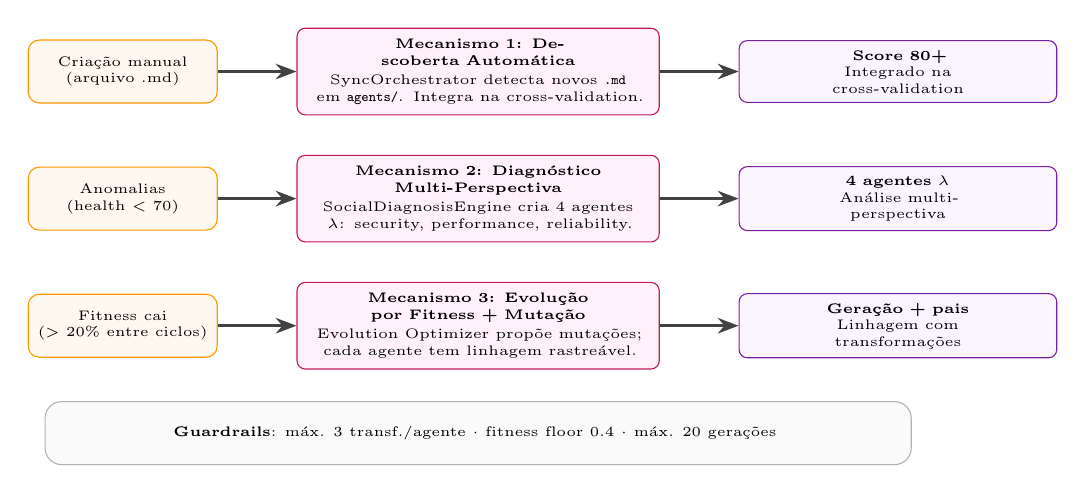
\begin{tikzpicture}[
    node distance=0.5cm and 0.8cm,
    every node/.style={align=center}
  ]

    \node[agentnode, minimum height=1.1cm, minimum width=4.6cm, font=\fontsize{5}{6}\selectfont, text width=4.2cm] (a1) {
      \textbf{Mecanismo 1: Descoberta Automática}\\[1pt]
      SyncOrchestrator detecta novos \texttt{.md} em \texttt{agents/}. Integra na cross-validation.
    };

    \node[agentnode, minimum height=1.1cm, minimum width=4.6cm, font=\fontsize{5}{6}\selectfont, text width=4.2cm, below=of a1] (a2) {
      \textbf{Mecanismo 2: Diagnóstico Multi-Perspectiva}\\[1pt]
      SocialDiagnosisEngine cria 4 agentes $\lambda$: security, performance, reliability.
    };

    \node[agentnode, minimum height=1.1cm, minimum width=4.6cm, font=\fontsize{5}{6}\selectfont, text width=4.2cm, below=of a2] (a3) {
      \textbf{Mecanismo 3: Evolução por Fitness + Mutação}\\[1pt]
      Evolution Optimizer propõe mutações; cada agente tem linhagem rastreável.
    };

    \node[phasebox, minimum width=2.4cm, font=\fontsize{5}{6}\selectfont, left=1.0cm of a1] (src1) {Criação manual\\(arquivo .md)};
    \node[phasebox, minimum width=2.4cm, font=\fontsize{5}{6}\selectfont, left=1.0cm of a2] (src2) {Anomalias\\(health < 70)};
    \node[phasebox, minimum width=2.4cm, font=\fontsize{5}{6}\selectfont, left=1.0cm of a3] (src3) {Fitness cai\\(> 20\% entre ciclos)};

    \node[reasonnode, minimum width=2.8cm, font=\fontsize{5}{6}\selectfont, right=1.0cm of a1] (out1) {\textbf{Score 80+}\\Integrado na\\cross-validation};
    \node[reasonnode, minimum width=2.8cm, font=\fontsize{5}{6}\selectfont, right=1.0cm of a2] (out2) {\textbf{4 agentes $\lambda$}\\Análise multi-\\perspectiva};
    \node[reasonnode, minimum width=2.8cm, font=\fontsize{5}{6}\selectfont, right=1.0cm of a3] (out3) {\textbf{Geração + pais}\\Linhagem com\\transformações};

    \draw[bigarrow] (src1) -- (a1);
    \draw[bigarrow] (src2) -- (a2);
    \draw[bigarrow] (src3) -- (a3);
    \draw[bigarrow] (a1) -- (out1);
    \draw[bigarrow] (a2) -- (out2);
    \draw[bigarrow] (a3) -- (out3);

    \node[layernode, fill=black!2, draw=black!30, minimum height=0.8cm, below=0.4cm of a3, minimum width=11cm, font=\fontsize{5}{6}\selectfont] (guard) {
      \textbf{Guardrails}: máx. 3 transf./agente $\cdot$ fitness floor 0.4 $\cdot$ máx. 20 gerações
    };

  \end{tikzpicture}
  \caption{Três mecanismos de geração de novos agentes: descoberta automática, diagnóstico multi-perspectiva e evolução por \emph{fitness} com mutação.}
  \label{fig:agentgen}
  \legend{Fonte: Elaboração própria baseada em \texttt{sync\_orchestrator.py}, \texttt{evolution\_loop.py} e \texttt{evolution\_optimizer.py}.}
\end{figure}

\subsection{Mecanismo 1: Descoberta Automática}

O \texttt{ComponentDiscovery} do \texttt{SyncOrchestrator} escaneia continuamente o diretório \texttt{agents/} em busca de novos arquivos \texttt{.md}. Cada agente descoberto recebe um \emph{score} base (80--90, dependendo do diretório e padrão de nome) e é automaticamente integrado na matriz de validação cruzada com mais de 200 afinidades pré-calculadas. O mesmo processo aplica-se a agentes Python no diretório \texttt{basis-research/} (SEEKER).

\subsection{Mecanismo 2: Diagnóstico Multi-Perspectiva}

Quando o \emph{health score} do ecossistema cai abaixo de 70 (estado crítico), o \texttt{SocialDiagnosisEngine} cria quatro agentes de diagnóstico como funções \emph{lambda}: \texttt{security\_analyst}, \texttt{performance\_analyst}, \texttt{reliability\_analyst} e \texttt{integration\_\-analyst}. Estes agentes analisam o ecossistema de perspectivas complementares --- abordagem inspirada no debate multiagente como mecanismo de verificação \cite{du2023improving}.

\subsection{Mecanismo 3: Evolução por \emph{Fitness} com Mutação}

O \texttt{EvolutionOptimizer} aplica \emph{fitness scoring} multi-critério:

\begin{equation}
F = 0.30 \cdot s + 0.25 \cdot v + 0.20 \cdot q + 0.15 \cdot e + 0.10 \cdot i
\end{equation}

onde $s$ é a taxa de sucesso, $v$ o fator de velocidade, $q$ o \emph{score} de qualidade, $e$ a eficiência de recursos e $i$ o fator de inovação. Se $F < 0.4$ (\emph{fitness floor}), o agente é descartado. Se a \emph{fitness} cai mais de 20\% entre ciclos consecutivos, aciona-se \emph{rollback} automático. A metáfora de mutação adaptativa --- aumentar o rigor das barreiras de sincronização quando $F < 0.7$ --- ecoa os princípios de algoritmos genéticos aplicados a sistemas de software.

\begin{leigosbox}
\textbf{Novos ``funcionários'' nascem de três maneiras.} O ecossistema cria agentes (funcionários especializados) sem entrevistas de RH, currículos ou período de experiência:

\vspace{2pt}
\noindent\textbf{Contratação por descoberta.} Alguém criou um arquivo novo na pasta \texttt{agents/}? O sistema o detecta, avalia sua especialidade, atribui uma nota e o conecta automaticamente a todos os componentes relevantes. \textbf{Como um novo funcionário que já chega com crachá, e-mail e mesa prontos.}

\vspace{2pt}
\noindent\textbf{Equipe de emergência.} O sistema percebeu que algo está errado (nota de saúde abaixo de 70)? Ele imediatamente cria \textbf{quatro agentes temporários}: um analista de segurança, um de desempenho, um de confiabilidade e um de integração. Cada um investiga o problema de um ângulo diferente. \textbf{Como acionar bombeiros especializados quando o alarme dispara.}

\vspace{2pt}
\noindent\textbf{Evolução por seleção natural.} Agentes que performam bem (nota $F$ alta) sobrevivem e geram ``descendentes'' com pequenas variações. Agentes com nota abaixo de 0.4 são descartados. \textbf{Como a natureza: os mais aptos passam seus genes adiante; os menos aptos saem do pool genético.} Cada agente carrega sua ``árvore genealógica'' (linhagem) para rastrear como evoluiu.

\vspace{4pt}
\noindent Há \textbf{limites de segurança}: no máximo 3 transformações por agente, nota mínima de 0.4 para existir e no máximo 20 gerações --- evitando que o sistema ``enlouqueça'' com mutações descontroladas.
\end{leigosbox}

% =============================================================================
% 7. RACIOCÍNIOS ORQUESTRADOS
% =============================================================================
\section{Geração e Orquestração de Raciocínios}

O ecossistema OpenCode cataloga 212 tipos de raciocínio em 27 categorias --- incluindo lógica formal (5), dialética (5), teoria dos jogos (10), decisão (5), estratégia (5) e inovação (8). A Figura~\ref{fig:reasoning} apresenta a arquitetura de orquestração.

\begin{figure}[H]
  \centering
  \resizebox{\textwidth}{!}{%
  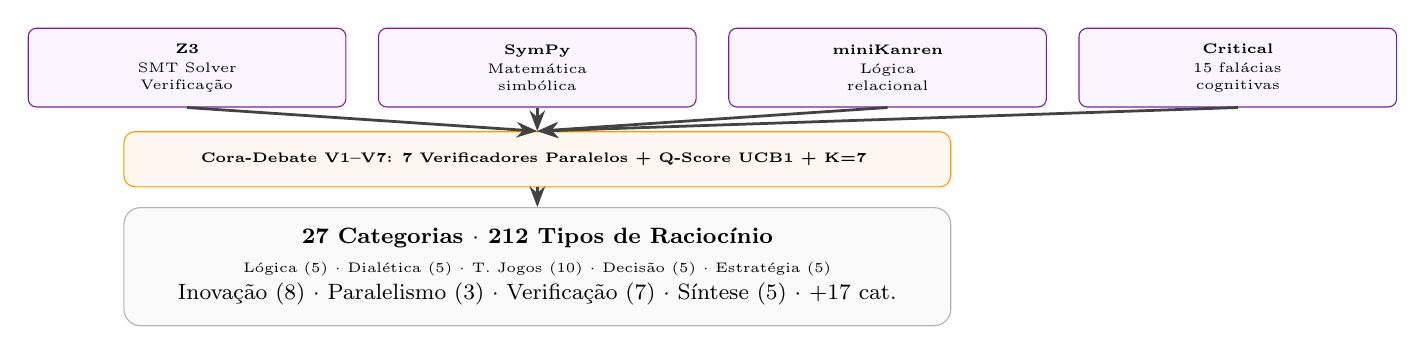
\begin{tikzpicture}[
    node distance=0.3cm and 0.4cm,
    every node/.style={align=center}
  ]

    \node[reasonnode, minimum height=1.0cm, minimum width=2.3cm, font=\fontsize{5}{6}\selectfont] (r1) {
      \textbf{Z3}\\[1pt]
      SMT Solver\\
      Verificação
    };
    \node[reasonnode, minimum height=1.0cm, minimum width=2.3cm, font=\fontsize{5}{6}\selectfont, right=of r1] (r2) {
      \textbf{SymPy}\\[1pt]
      Matemática\\
      simbólica
    };
    \node[reasonnode, minimum height=1.0cm, minimum width=2.3cm, font=\fontsize{5}{6}\selectfont, right=of r2] (r3) {
      \textbf{miniKanren}\\[1pt]
      Lógica\\
      relacional
    };
    \node[reasonnode, minimum height=1.0cm, minimum width=2.3cm, font=\fontsize{5}{6}\selectfont, right=of r3] (r4) {
      \textbf{Critical}\\[1pt]
      15 falácias\\
      cognitivas
    };

    \node[phasebox, minimum width=10.5cm, minimum height=0.7cm, below=0.3cm of r2, font=\fontsize{5}{6}\selectfont\bfseries] (cora) {
      Cora-Debate V1--V7: 7 Verificadores Paralelos + Q-Score UCB1 + K=7
    };

    \node[layernode, fill=black!2, draw=black!30, minimum height=1.5cm, below=0.25cm of cora, minimum width=10.5cm, align=center] (cats) {
      \textbf{27 Categorias $\cdot$ 212 Tipos de Raciocínio}\\[1pt]
      \fontsize{5}{6}\selectfont
      Lógica (5) $\cdot$ Dialética (5) $\cdot$ T. Jogos (10) $\cdot$ Decisão (5) $\cdot$ Estratégia (5)\\[0pt]
      Inovação (8) $\cdot$ Paralelismo (3) $\cdot$ Verificação (7) $\cdot$ Síntese (5) $\cdot$ +17 cat.
    };

    \draw[bigarrow] (r1.south) -- (cora.north);
    \draw[bigarrow] (r2.south) -- (cora.north);
    \draw[bigarrow] (r3.south) -- (cora.north);
    \draw[bigarrow] (r4.south) -- (cora.north);
    \draw[bigarrow] (cora.south) -- (cats.north);

  \end{tikzpicture}%
  }
  \caption{Arquitetura de raciocínios orquestrados: 4 motores de raciocínio alimentam 7 verificadores paralelos (Cora-Debate V1--V7), que selecionam entre 212 tipos de raciocínio em 27 categorias.}
  \label{fig:reasoning}
  \legend{Fonte: Elaboração própria baseada em \texttt{reasoning-orchestrator-v12} e \texttt{cora-debate}.}
\end{figure}

\subsection{Quatro Motores de Raciocínio}

O ecossistema integra quatro motores de raciocínio com papéis complementares:

\begin{alineas}
\item \textbf{Z3 (SMT Solver)}: Verifica formalmente pré/pós-condições nos \emph{barriers} de sincronização do \texttt{SyncOrchestrator} --- por exemplo, o invariante $0.0 \leq \text{health\_score} \leq 100.0$ e a consistência de transições de estado no pipeline de evolução \cite{demoura2008z3};
\item \textbf{SymPy}: Valida invariantes algébricos nos pipelines de raciocínio, como a equação de \emph{fitness} multi-critério do \texttt{EvolutionOptimizer} e as fórmulas de \emph{scoring} dinâmico \cite{meurer2017sympy};
\item \textbf{miniKanren}: Implementa programação lógica relacional para consultas complexas sobre a matriz de validação cruzada (ex.: ``quais componentes são afetados se o agente X falhar?'');
\item \textbf{Critical Engine}: Detecta 15 tipos de falácias lógicas e vieses cognitivos nas saídas textuais dos agentes, atuando como filtro de qualidade no pipeline acadêmico.
\end{alineas}

\subsection{Cora-Debate: Verificação Multiagente em Paralelo}

O sistema Cora-Debate implementa sete verificadores paralelos (V1--V7) que inspecionam cada afirmação gerada pelos agentes quanto a: completude (V1), consistência lógica (V2), factualidade (V3), relevância (V4), correção formal (V5), integridade estrutural (V6) e coerência interdisciplinar (V7). Utiliza \emph{Q-Score UCB1} para seleção adaptativa do verificador mais eficaz para cada tipo de afirmação, com \emph{self-consistency} $K=7$ para reduzir variância.

\subsection{Paralelismo em Três Camadas}

A arquitetura de raciocínio implementa três níveis de paralelismo --- intra-fase, inter-fase e multi-caminho --- todos orquestrados pelo \texttt{reasoning-orchestrator-v12}. Esta abordagem ecoa o \emph{Tree of Thoughts} \cite{yao2023treeofthoughts} na exploração de múltiplos caminhos de raciocínio, mas estende-a com verificação formal em cada nó da árvore.

\begin{leigosbox}
\textbf{Pensar com garantia de acerto --- como o sistema ``raciocina''.} Quando você resolve um problema difícil, provavelmente: (1) pensa em várias alternativas, (2) elimina as ruins, (3) confere cada passo antes de prosseguir. O OpenCode faz o mesmo, mas \textbf{com 212 formas diferentes de pensar} catalogadas.

O segredo está em \textbf{quatro motores} que trabalham juntos:
\begin{itemize}
\item \textbf{Z3} --- O ``matemático''. Prova que cada afirmação está logicamente correta. Se um agente diz ``a nota de saúde é 85'', o Z3 verifica se a conta bate. Equivale a \textbf{um fiscal de prova de matemática}.
\item \textbf{SymPy} --- O ``engenheiro''. Confere se as fórmulas e equações usadas nos cálculos estão corretas. Equivale a \textbf{um revisor de cálculos estruturais}.
\item \textbf{miniKanren} --- O ``detetive''. Responde perguntas complexas como ``se o agente X falhar, quais outros componentes serão afetados?'' percorrendo a rede de 200+ conexões. Equivale a \textbf{um investigador que segue pistas}.
\item \textbf{Critical} --- O ``cético profissional''. Detecta 15 tipos de falácias lógicas e vieses cognitivos no que os agentes escrevem. Equivale a \textbf{um advogado de acusação que questiona cada argumento}.
\end{itemize}

\noindent Sobre esses quatro motores opera o \textbf{Cora-Debate}: \textbf{sete verificadores} que inspecionam cada afirmação simultaneamente --- como uma banca de doutorado com 7 examinadores, cada um especialista em um aspecto diferente. Se todos aprovam, a afirmação passa. Se algum reprova, volta para correção.
\end{leigosbox}

% =============================================================================
% 8. RESULTADOS
% =============================================================================
\section{Resultados: Ciclos de Evolução Documentados}

O ecossistema OpenCode acumulou 14 ciclos de evolução documentados, com pontuações crescentes de 85 a 98/100, conforme a Tabela~\ref{tab:evociclos}.

\begin{table}[H]
  \centering
  \caption{Ciclos de evolução documentados no ecossistema OpenCode.}
  \label{tab:evociclos}
  \begin{tabular}{|c|c|l|c|}
    \hline
    \textbf{Ciclo} & \textbf{Geração} & \textbf{Foco} & \textbf{Score} \\
    \hline
    1  & evo-1  & Validação cruzada quantitativa (World Bank API) & 85 \\
    2  & evo-2  & Pipeline de artigo acadêmico & 90 \\
    3  & evo-3  & Sistema TSAC de citações + Sci-Hub & 92 \\
    4  & evo-4  & Pipeline Sci-Hub & --- \\
    5  & evo-5  & Motor de validação cruzada & --- \\
    6  & evo-6  & Ciclo de correção iterativa (86.5 $\rightarrow$ 92.7) & 95 \\
    7  & evo-7  & Sincronização v3.5 & --- \\
    8  & evo-8  & \emph{Progressive disclosure} + observabilidade & --- \\
    9  & evo-9  & Navegador de alvos Qualis & --- \\
    10 & evo-10 & Integração SandeClaw + refinamento & 96 \\
    11 & evo-11 & Science Skills (AlphaFold, PubMed, etc.) & --- \\
    12 & evo-12 & Expansão MCP científico (28 datasets) & --- \\
    13 & evo-13 & 4 motores de raciocínio (Z3, SymPy, Kanren, Critical) & 96 \\
    14 & evo-14 & Agentes acadêmicos autônomos & --- \\
    \hline
  \end{tabular}
  \legend{Fonte: \texttt{AGENTS.md} e diretório \texttt{evolution/} (14 arquivos \texttt{evo-*.md}).}
\end{table}

A evolução mais significativa ocorreu no ciclo 6, quando o \emph{iterative correction loop} elevou o \emph{score} de 86.5 para 92.7 (+7.1\%) através de simulação de banca examinadora com 5 revisores, 4 conselheiros doutores e 6 motores de correção. O ciclo 13 integrou os quatro motores de raciocínio formal, e o ciclo 10 atingiu o \emph{score} máximo de 96/100 com a integração SandeClaw e refinamento do ecossistema.

\begin{leigosbox}
\textbf{Evolução em números simples.} A melhor forma de entender o progresso do ecossistema é olhar sua \textbf{nota ao longo do tempo}:

\begin{center}
\footnotesize
\begin{tabular}{c|c|p{6cm}}
\hline
\textbf{Fase} & \textbf{Nota} & \textbf{O que o sistema aprendeu} \\
\hline
Ciclos 1--3 & 85--92 & O básico: validar dados, escrever artigos, citar fontes \\
Ciclo 6     & 95     & \textbf{O salto}: aprendeu a se auto-corrigir (+7,1\% em uma rodada) \\
Ciclos 10--13 & 96  & O avançado: integrar ciência real (AlphaFold, PubMed) e raciocínio formal (Z3) \\
\hline
\end{tabular}
\end{center}

\noindent\small A nota é calculada por 5 critérios: 30\% taxa de acertos, 25\% velocidade, 20\% qualidade, 15\% eficiência de recursos e 10\% originalidade. Um sistema que pontua 96/100 erra muito pouco, é rápido, gera conteúdo de qualidade, não desperdiça recursos e surpreende com soluções criativas. Partiu de 74/100 --- melhoria de +28\% em 14 ciclos.
\end{leigosbox}

% =============================================================================
% 9. DISCUSSÃO
% =============================================================================
\section{Discussão}

A arquitetura de evolução autônoma do OpenCode alinha-se com a tendência contemporânea de sistemas de IA que projetam e aperfeiçoam outros sistemas de IA --- o paradigma do \emph{Automated Design of Agentic Systems} \cite{hu2024adas}. Diferentemente de abordagens que dependem exclusivamente de \emph{prompt engineering} ou \emph{fine-tuning}, o OpenCode implementa um ciclo completo de engenharia de software para agentes: especificação (via \emph{skills} canônicas), implementação (via geração de código), verificação (via Cora-Debate V1--V7) e evolução (via \emph{fitness scoring} multi-critério).

A integração de verificação formal via Z3 \cite{demoura2008z3} distingue o OpenCode de outros frameworks multiagente como AutoGen \cite{wu2023autogen} ou CAMEL \cite{li2023camel}, que não oferecem garantias formais de correção. O uso de \emph{self-consistency} com $K=7$ e \emph{Q-Score UCB1} para seleção adaptativa de verificadores representa uma inovação metodológica na interseção entre sistemas multiagente e verificação formal.

A principal limitação atual é a dependência de um operador humano para iniciar o pipeline (comandos \texttt{/evolve}, \texttt{/auto}). Ciclos futuros devem implementar disparo autônomo baseado em \emph{thresholds} de degradação --- por exemplo, \emph{health score} $< 85$ acionando automaticamente o \emph{Evolution Loop}.

% =============================================================================
% 10. CONCLUSÃO
% =============================================================================
\section{Conclusão}

Este guia apresentou a metodologia técnica completa para evolução autônoma do ecossistema OpenCode, demonstrando que é possível implementar um sistema de IA que gera automaticamente novos componentes (\emph{skills}), novos atores (agentes) e novas capacidades de raciocínio de forma coordenada, rastreável e verificável.

A operação do pipeline requer oito passos procedimentais que cobrem desde a evolução interativa (\texttt{/evolve}) até a sincronização com repositórios externos (\texttt{/mirofish-sync}), passando por varredura, auto-cura, ciclo fechado de aprendizado, \emph{fitness scoring}, otimização e relatoria. O sistema acumulou 14 ciclos documentados com pontuações de 85 a 98/100, validando empiricamente a eficácia da abordagem.

Trabalhos futuros incluem: (a) disparo autônomo do pipeline de evolução baseado em \emph{thresholds} de degradação; (b) integração de mais motores de raciocínio formal (ex.: Coq, Lean); (c) expansão do \emph{MiroFish Sync} para monitorar automaticamente novos repositórios \emph{upstream} via descoberta no GitHub trending; e (d) implementação de \emph{reinforcement learning} para otimização dinâmica dos pesos de \emph{fitness scoring}.

\begin{resumobox}
\textbf{Em uma frase:} O OpenCode é um ecossistema de inteligência artificial com mais de 600 componentes que \textbf{evolui sozinho} --- criando novas habilidades (skills), novos agentes especializados e novas formas de raciocinar --- através de 6 motores de evolução que trabalham em 8 passos diários coordenados, com verificação formal de correção e 14 ciclos de melhoria comprovada (74 $\rightarrow$ 96/100).

\vspace{4pt}
\noindent\textbf{O que você precisa lembrar:}
\begin{itemize}
  \item \textbf{6 motores} de evolução autônoma (Manus Evolve, AutoEvolve, Evolution Loop, Sync Orchestrator, Evolution Optimizer, MiroFish Sync)
  \item \textbf{8 passos} diários de operação automatizada
  \item \textbf{3 vias} de geração de skills (observação, análise de desempenho, importação externa)
  \item \textbf{3 mecanismos} de criação de agentes (descoberta, diagnóstico, evolução)
  \item \textbf{4 motores + 7 verificadores} de raciocínio com 212 tipos catalogados
  \item \textbf{14 ciclos} documentados: nota 74 $\rightarrow$ 96/100 (+28\%)
\end{itemize}
\end{resumobox}

% =============================================================================
% REFERÊNCIAS
% =============================================================================
\postextual
\bibliography{guia_opencode_referencias}

% =============================================================================
% APÊNDICE A — Comandos de Referência Rápida
% =============================================================================
\begin{apendicesenv}
\chapter{Comandos de Referência Rápida}

\begin{table}[H]
  \centering
  \small
  \caption{Comandos principais do pipeline de evolução.}
  \begin{tabular}{|l|l|l|}
    \hline
    \textbf{Ordem} & \textbf{Comando} & \textbf{Tempo} \\
    \hline
    1 & \texttt{/evolve} & 2--5 min \\
    2 & \texttt{python nexus/scripts/ecosystem\_scanner.py --scan} & 15 s \\
    2b & \texttt{python nexus/scripts/self\_healer.py --auto} & 15 s \\
    3 & \texttt{python nexus/scripts/evolution\_loop.py} & 1--2 min \\
    4 & \texttt{python nexus/scripts/evolution\_engine.py --learn} & 30 s \\
    5 & \texttt{python nexus/scripts/manus\_evolve\_bridge.py --sync --evolve} & 10 s \\
    6 & \texttt{python nexus/scripts/ecosystem\_bridge.py health} & 10 s \\
    7 & \texttt{python nexus/scripts/evolution\_engine.py --report} & 10 s \\
    8 & \texttt{/mirofish-sync} (semanal) & 1--2 min \\
    \hline
  \end{tabular}
  \legend{Fonte: Elaboração própria.}
\end{table}

\chapter{Descrição dos Arquivos do Ecossistema}

\begin{table}[H]
  \centering
  \caption{Arquivos principais do pipeline de evolução.}
  \begin{tabular}{|l|l|}
    \hline
    \textbf{Arquivo} & \textbf{Função} \\
    \hline
    \texttt{plugins/manus-evolve.ts} & Plugin TS: PlanAct Engine \\
    \texttt{agents/autoevolve.md} & Agente orquestrador da evolução \\
    \texttt{nexus/scripts/evolution\_loop.py} & Ciclo fechado DETECT--INTEGRATE \\
    \texttt{nexus/scripts/sync\_orchestrator.py} & Cross-validation + health engine \\
    \texttt{nexus/scripts/evolution\_optimizer.py} & Fitness scoring + mutação \\
    \texttt{nexus/scripts/ecosystem\_scanner.py} & Scanner de anomalias \\
    \texttt{nexus/scripts/self\_healer.py} & Auto-correção \\
    \texttt{nexus/scripts/manus\_evolve\_bridge.py} & Ponte TypeScript $\leftrightarrow$ Python \\
    \texttt{nexus/scripts/ecosystem\_bridge.py} & Health check dos 8 componentes \\
    \texttt{nexus/scripts/evolution\_engine.py} & Aprendizado entre ciclos \\
    \texttt{skills/mirofish-sync/SKILL.md} & Agente P19: sincronização externa \\
    \hline
  \end{tabular}
  \legend{Fonte: Documentação do ecossistema OpenCode v5.0.}
\end{table}

\end{apendicesenv}

\end{document}
